\documentclass[11pt,english]{article}
\usepackage[T1]{fontenc}
\usepackage{babel}
\usepackage{graphicx}
\usepackage{epstopdf}
\usepackage[top=1in, bottom=1in, left=0.5in, right=0.5in]{geometry}
\usepackage{verbatimbox}
\author{
                Sanket Kanjanlkar\\
                120050011\\
                sanket@cse.iitb.ac.in
                \and 
                Shirish Namdeo\\
                110050040\\
                shirishkumar@cse.iitb.ac.in
                \and
                Pratyaksh Sharma\\
                120050019\\
                pratyaksh@cse.iitb.ac.in
}
\title{Timing and Profiling CS296 Base Code}
\date{1 March, 2014}
\begin{document}
\maketitle
\section{Timing}
\subsection{Introduction}
\indent \par{For the following analysis, we have used no. of iterations = 1500 and no. of reruns = 150.}
\subsection{Analysis of Loop time vs No. of iterations}
\begin{figure}[h!]
\centering
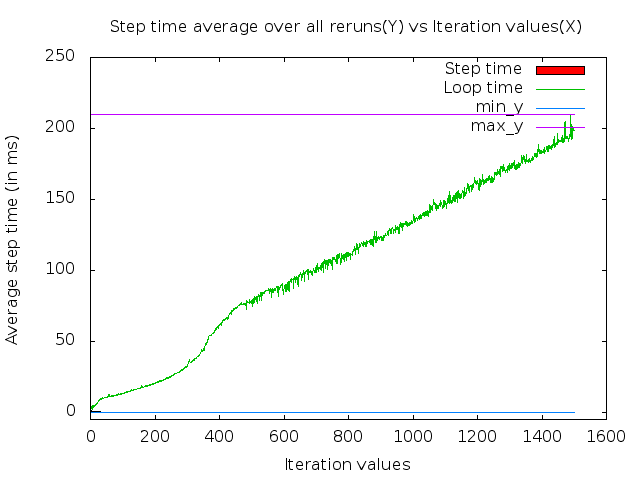
\includegraphics[scale=.45]{g09_plot01.png}
\caption{g09\_plot01}
\end{figure}
\indent \par{
The average step time almost remains constant. We obtain more accurate data as we take further iterations into account.} 
\indent \par{The total loop time increases almost linearly. There are some ups and downs in the line graph which indicates that the solver is only invoked when it is needed. In some particular iteration, where more collisions occur (and/or more objects move) take longer time for solver to solve and hence there is some variation in the (almost) linear loop time.}
\subsection{Observations from graph of Step time, Collision time, Velocity time, Position time vs Iteration values}
\begin{figure}[h!]
\centering
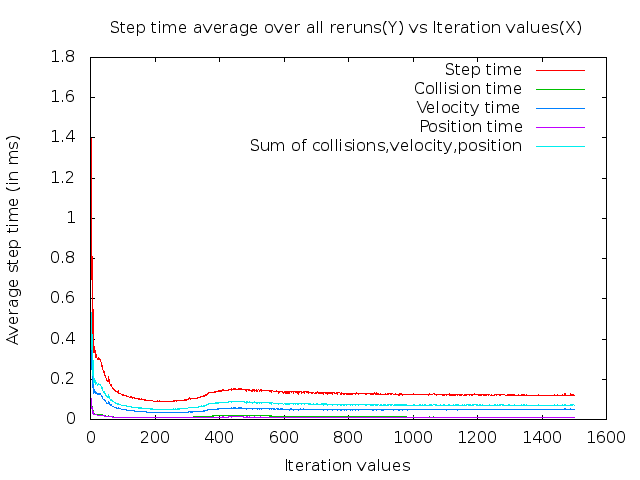
\includegraphics[scale=.45]{g09_plot02.png}
\caption{g09\_plot02}
\end{figure}
\indent \par{Box2D uses constraint solver for solving constraints. The constraint solver solves all the constraints in the simulation, one at a time. Although single constraint can be solved perfectly, when we solve one constraint, we slightly disrupt other constraints. Therefore to get a good solution, we need to iterate over all constraints a number of times (in the same time step).}

\indent \par{The time step and the iteration count are completely unrelated. An iteration is not a sub-step. One solver iteration is a single pass over all the constraints within a time step.
There are two phases in the constraint solver: a velocity phase and a position phase. Each phase has its own iteration count. Here we are used velocity iterations=8 and position iterations=3.}

\indent \par{
This creates a trade-off between speed and accuracy. Using fewer iterations increases performance but accuracy suffers. Likewise, using more iterations decreases performance but improves the quality of your simulation. Since velocity iterations are more than position iterations, this acts as one of the factors in due to which time taken for velocity solving is more than that for position solving.
}
\subsection{Observations from above two graphs}
\indent \par{From graphs 1 and 2 we can note that loop time lies below the average loop time and step time lies below the average time until iteration number is approx. 400. In our simulation on the iterations near 400, suddenly multiple collisions occur (the point when the last falling domino hits the set of balls on the platform) and moving objects also increase. Thereafter, as the iteration value increases all characteristics (vel\_time ,pos\_time ,collision time,loop time)  remain almost constant.}

\subsection{Observations from Step time average (error bars) vs No. of Iterations graph}
\begin{figure}[h!]
\centering
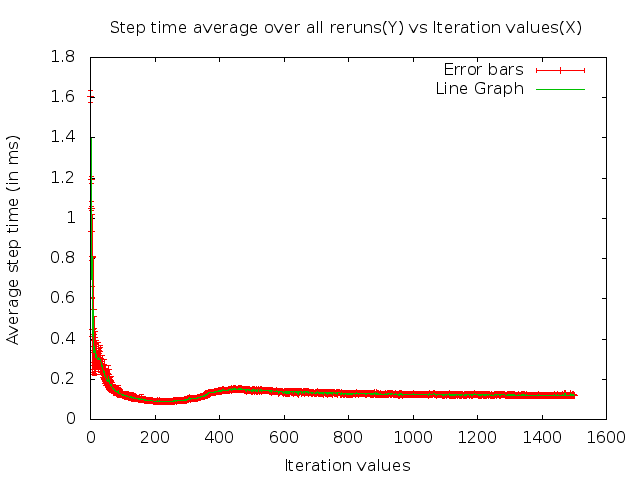
\includegraphics[scale=.45]{g09_plot03}
\caption{g09\_plot03}
\end{figure}
\indent \par{Note that the above plots represents average step time and y-error bars , the difference between the max and min values is large. Although the values are taken within 150 reruns, there are theses differences due to system processes. As the data is very large, error remains uniform over large values.}
\subsection{Effect of different types of system load}
\indent \par{a) When memory heavy processes are running, and the process has less available memory to run. The system tries to free some memory by killing other processes. Since processor may still be idle, the running time is not significantly affected.
b) When CPU heavy processes are running, the execution time increases significantly. This is because less processor cycles are used towards a particular process.
}
\indent \par{Observations for 10000 iterations:} 
Normal (8\% CPU,16\% mem usage) 1.572s \\
CPU load (97\% CPU,20\% mem usage) 2.208s \\
RAM load (12\% CPU, 91\% mem usage) 1.625s \\
CPU and RAM load (92\% CPU, 91\% mem usage) 2.856s
\subsection{gettimeofday() vs time}
\indent \par{\verb+time+ writes a message to standard output giving timing statistics about this program run. \\
Real time: the elapsed real time between invocation and termination, \\
User time: the user CPU time \\
System time: the system CPU time}
The user time tells us how long your program was running on the CPU. The system time tells how long  the program was waiting for the OS to perform the given tasks for it. Real time: This is the actual time difference between starting and ending of program. This can be affected by other running processes. The Unix time command measures the whole program execution time, including the time it takes for the system to load your binary and all its libraries, and the time it takes to clean up everything once your program is finished. 
\indent \par{Gettimeofday can only work inside your program, that is after it has been initialized, and before it is terminated.}
\section{Profiling}
\subsection{perf}
\indent
\par{The profiler used for this task is \verb+perf+. The command \verb+perf report ./mybins/cs296_09_exe+ runs the executable and records samples required for profiling in a file \verb+perf.data+. To generate human readable flat profile, the command \verb+perf record+ is used.}
\subsection{Release mode}
\indent 
\par{For profiling in this mode, we use the \verb+cmake -DCMAKE_BUILD_TYPE=Release ../.+ command in Box2D installation. This is an out-of-source build.  An out-of-source build puts the files generated by the built in a completely separate directory, so that the source tree is unchanged. Also, the \verb+-O3+ flag is used with \verb+gcc+ in code compilation.}
\subsubsection{O3 compiler optimization}
\indent 
\par{Turning on optimization flags makes the compiler attempt to improve the performance and/or code size at the expense of compilation time and possibly the ability to debug the program. The \verb+-O3+ flag uses all the optimizations used by the \verb+-O2+ flag and a few more. An important one of them is that it inlines functions. This means that the compiler inserts the body of a function wherever it is called. This obviously reduces function calls and associated overheads, thus making the program faster (at the expense of increasing the size of the executable). }
\subsubsection{Profiling Report}
\indent 
\par{The executable \verb+./mybins/cs296_09_exe+ was run with 5000 iterations of the for loop, and the output of \verb+perf report+ is shown in Figure 1. }
\indent
\par{The function which which makes up a large part of the running time is \verb+0x2cfd0+. Other hexadecimal values like \verb+0x7fff81fff797+, \verb+0x11006+ etc. can be seen. As we had compiled our program in release mode and had used \verb+-O3+ compiler optimization, our ability to debug the program has reduced (the takeoff is between speed and debugging ability). This leads to perf being unable to resolve the calls to function names.} 
\indent \par{Also, a number of functions have been inlined (because of \verb+-O3+ optimization flag), so the function calls in the code have been replaced by the functions body. This means that the (percentage of) samples collected of the parent function will include the samples that should have been collected of the called function.}
\indent \par{The column 'Overhead' indicates the percentage of the overall samples collected in the corresponding function. The second column reports the process from which the samples were collected. If a program is dynamically linked, then this shows the name of a shared library. When the samples come from the kernel, then the pseudo ELF image name [kernel.kallsyms] is used.}
\begin{figure}[h!]
\centering
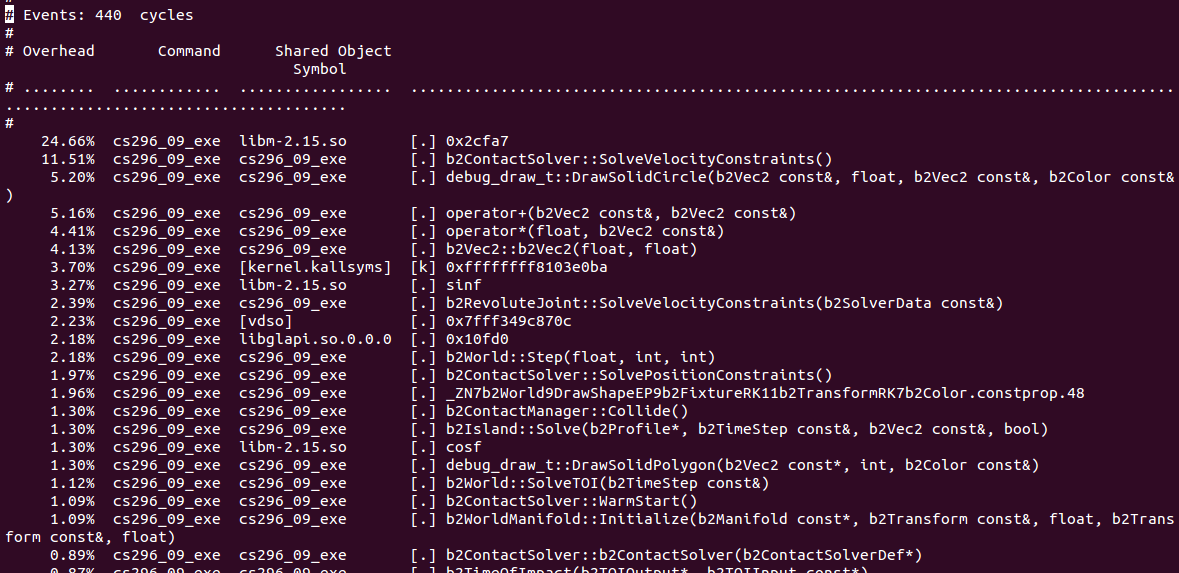
\includegraphics[scale=.33]{release_report}
\caption{perf report in Release mode.}
\end{figure}
\subsubsection{Call graph}
\indent 
\par{Using \verb+perf record -g -- ./mybins/cs296_09_exe+, call-graph recording is written (along with the flat profile) to \verb+perf.data+. Running \verb+perf script | ./gprof2dot.py -f perf | dot -Tpng -o release.png+ generates a call-graph image, part of which is shown in Figure 5.}
\begin{figure}[h!]
\centering
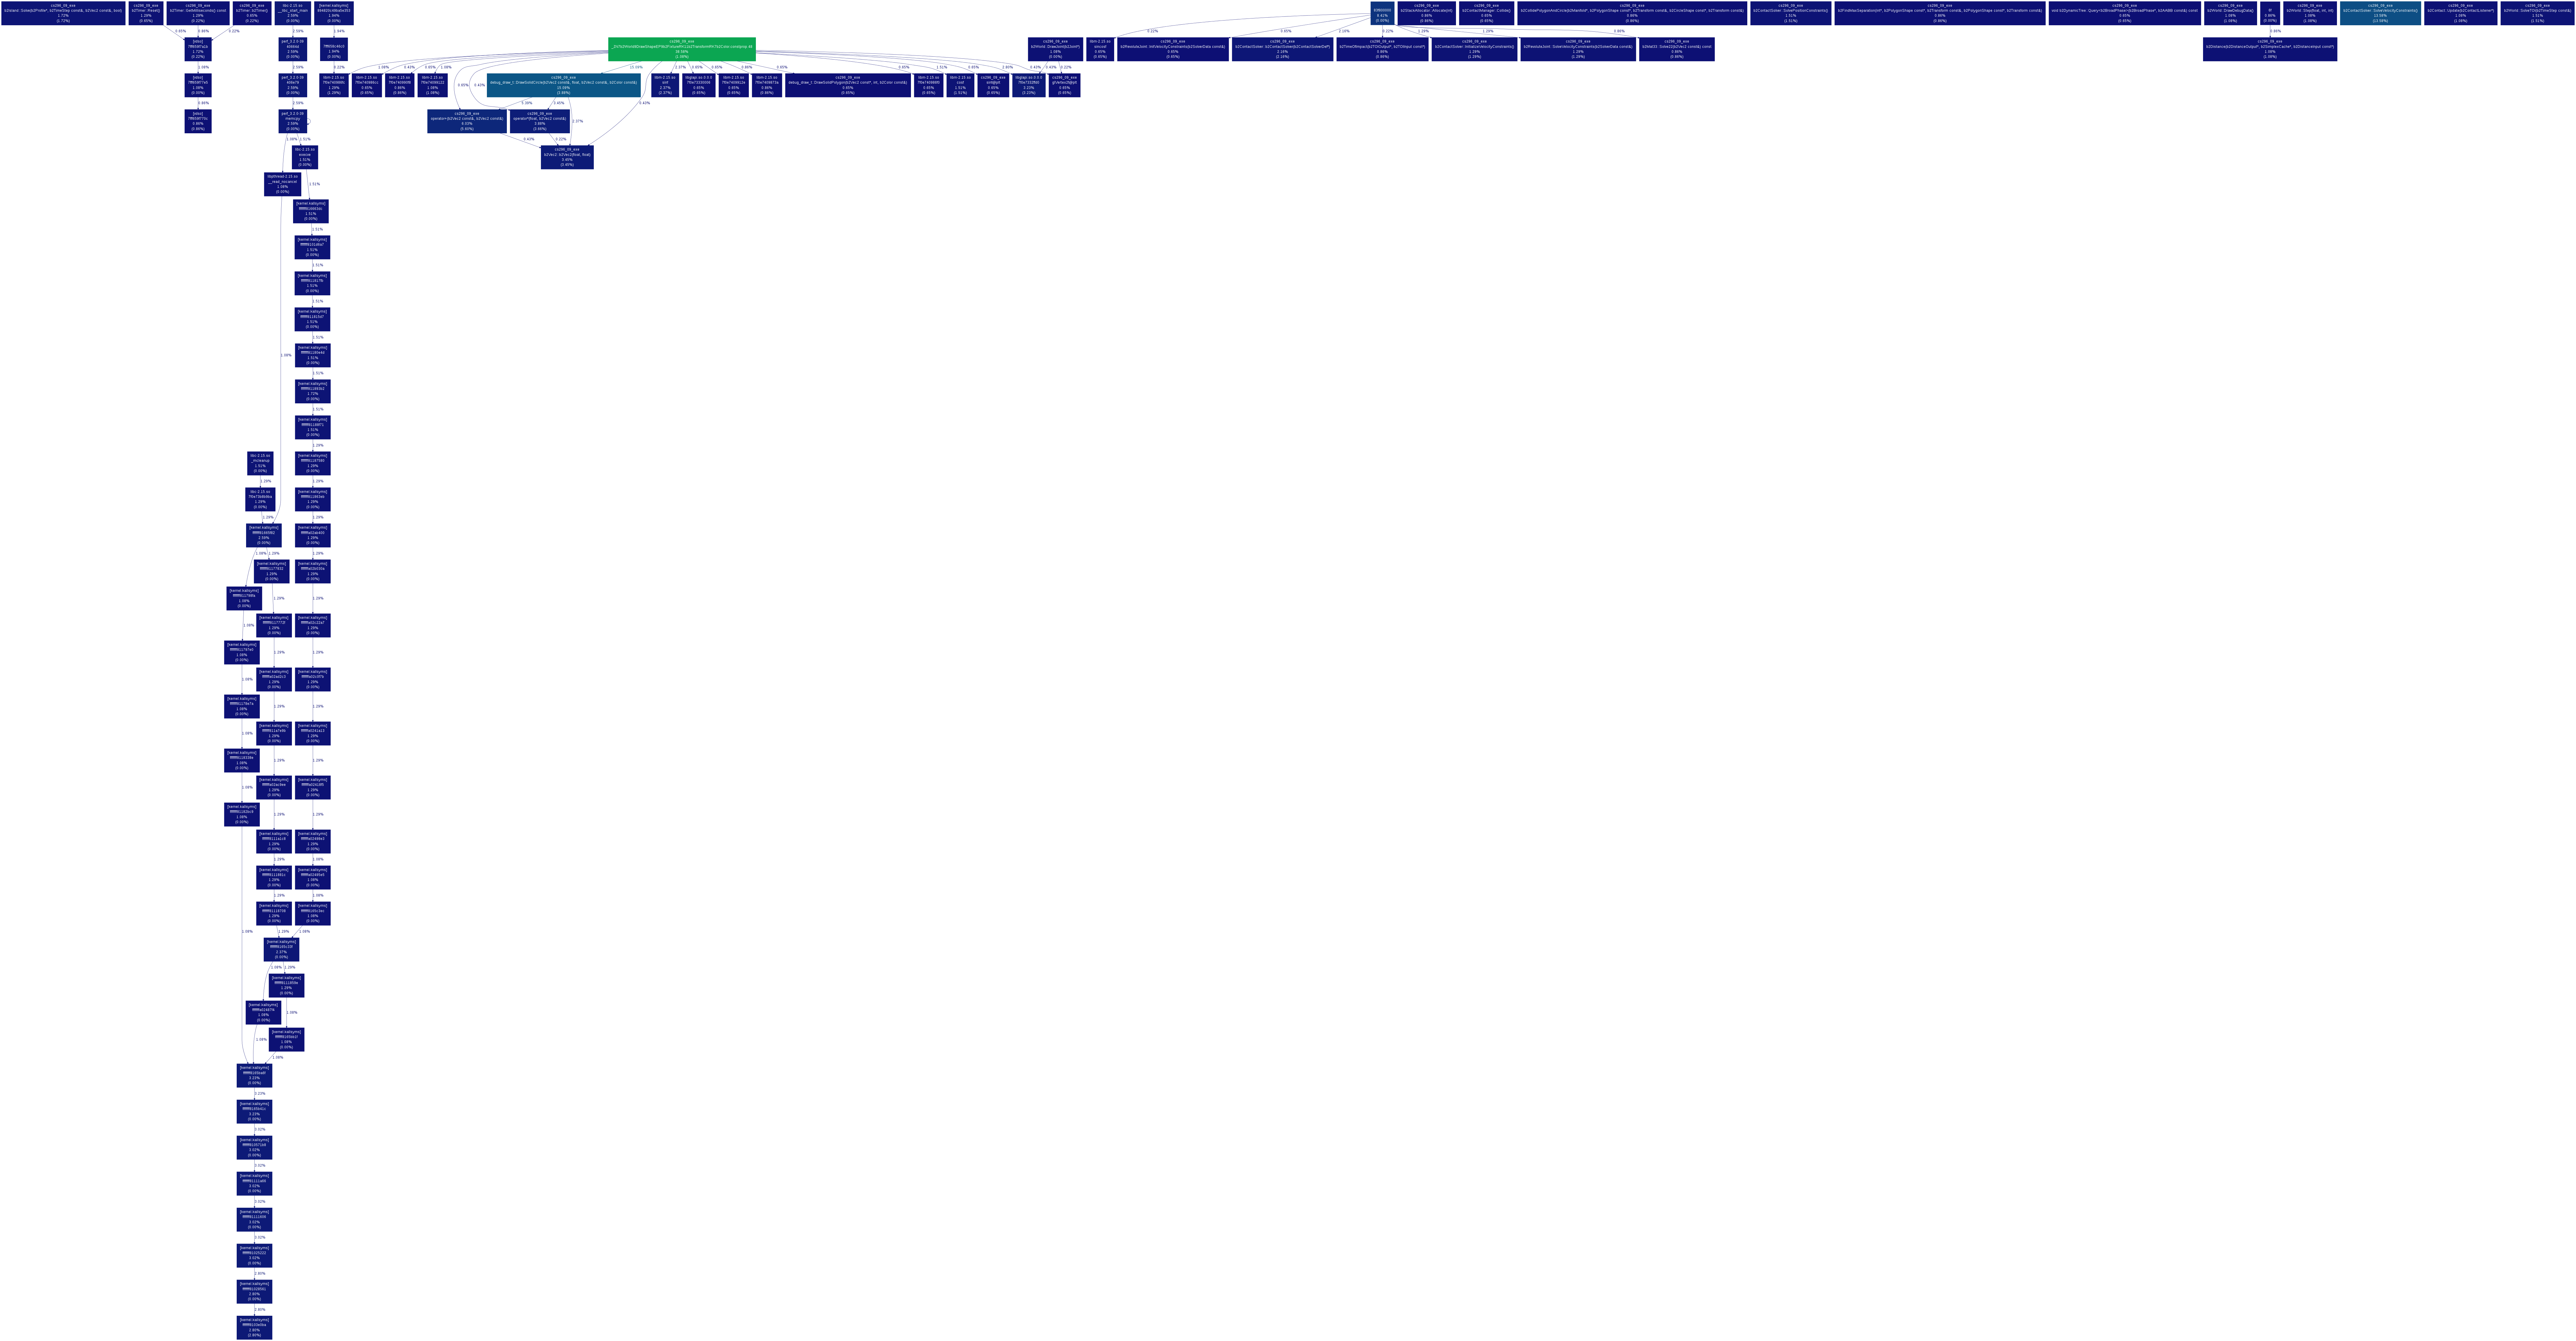
\includegraphics[scale=.05]{release_callgraph}
\caption{Call graph in release mode.}
\end{figure}
\indent
\par{A node in the output graph represents a function and has the following layout: 
\begin{verbatim}
             +------------------------------+
             |        function name         |
             |        total time %          |
             |        ( self time % )       |
             +------------------------------+
\end{verbatim}
where total time\% is the percentage of the running time spent in this function and all its children; self time \% is the percentage of the running time spent in this function alone.
}
\indent \par{An edge represents the calls between two functions and has the following layout: 
\begin{verbatim}
                        total time %
             parent --------------------> children
\end{verbatim}
Where total time \% is the percentage of the running time transfered from the children to this parent (if available).
}
\par{This call-graph is quite complicated, but it is clear that it has few levels of function calls (except in one branch). This is again because of the various compiler optimizations used.}
\subsection{Debugging mode}
\par{\verb+cmake -DCMAKE_BUILD_TYPE=Debug+ has been used in Box2D installation. This uses various debugging flags of the compiler. Also, compiler optimization options have been excluded. This means the debugging of the program will be easier, but at the expense of speed.}
\subsubsection{Profiling report}
\indent \par{The executable \verb+./mybins/cs296_09_exe+ was run with 5000 iterations of the for loop, and the output of \verb+perf report+ is shown in Figure 6. }
\begin{figure}[h]
\centering
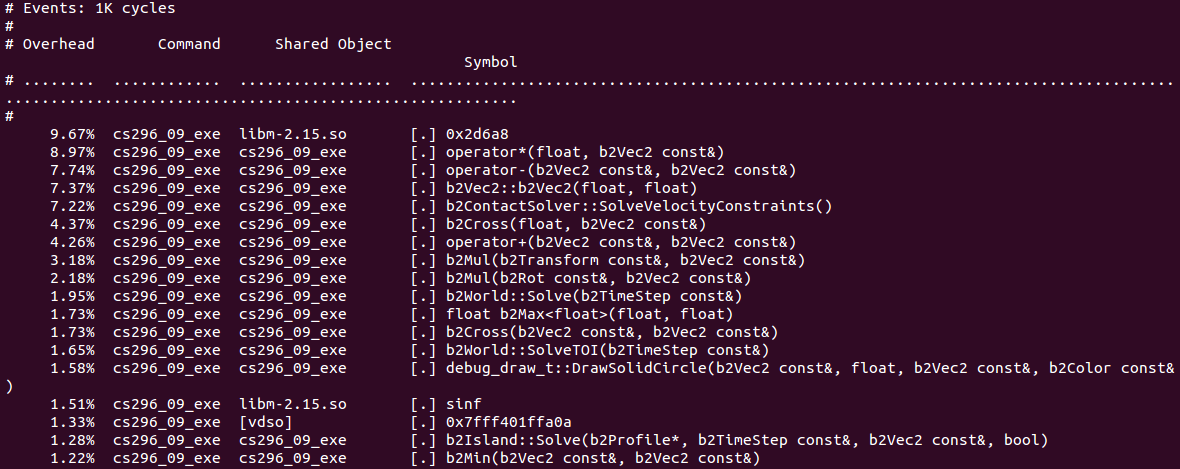
\includegraphics[scale=.33]{debug_report}
\caption{perf report in Debug mode.}
\end{figure}
\indent \par{This report is clearer than that produced in release mode. The highest overhead is from symbol \verb+0x2d6a8+, which is from the libm-2.15.so shared object. Other function calls whose overhead is high are: \verb^operator*^, \verb^operator+^, \verb^operator-^, \verb^b2ContactSolver^, \verb^b2Vec^ etc. We must focus on optimizing (or reducing their number of calls of) the latter functions (which are part of Box2D), rather than trying to optimize the function \verb+0x2d6a8+, which is from a dynamic library.}
\subsubsection{Call graph}
\indent \par{The call graph generated is shown in Figure 7. It can be easily seen that this has higher number of function calls (because compiler optimization options have not been used). Also, this graph is easier to understand (and to debug) than that produced in Release mode. Familiar functions like \verb+main+, \verb+b2ContactSolver+, \verb+b2World::Step+ etc. can be identified easily.}
\begin{figure}[h!]
\centering
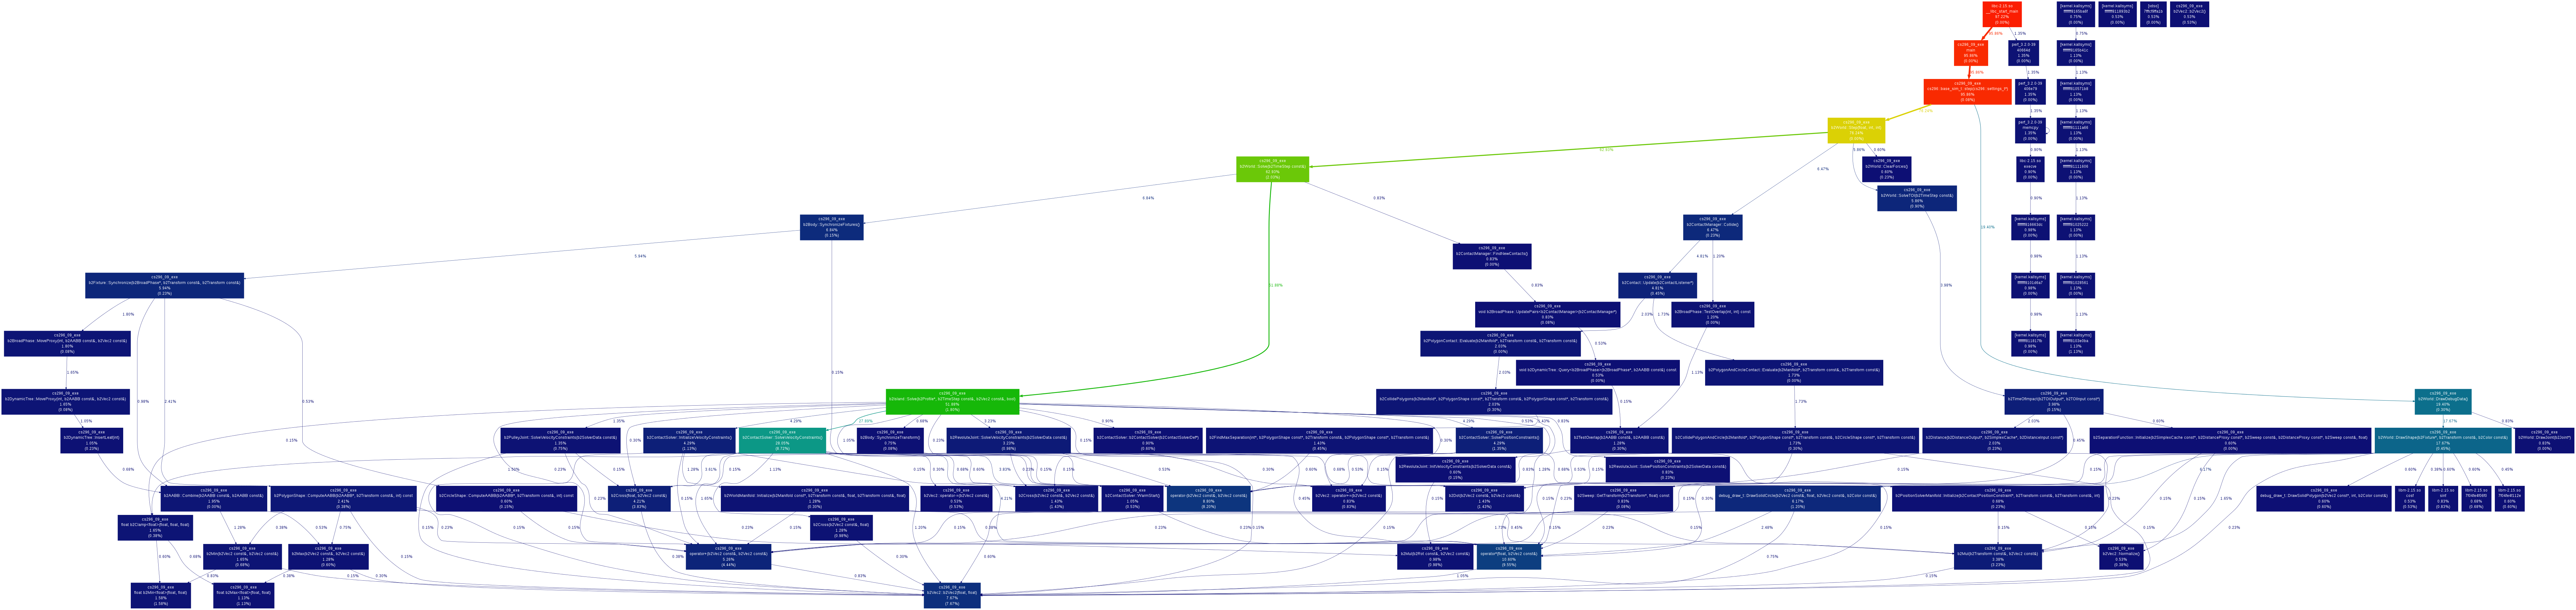
\includegraphics[scale=.06]{debug_callgraph}
\caption{Call graph in Debug mode.}
\end{figure}
\end{document}
